% BEGIN
% ETH STYLE -> DON'T CHANGE
\documentclass[british,11pt,a4paper]{memoir}
\usepackage[utf8]{inputenc}
\usepackage[OT1]{fontenc}
\usepackage{babel}
\usepackage[sc]{mathpazo}
\usepackage{amsmath,amssymb,amsfonts,mathrsfs}
\usepackage[amsmath,thmmarks]{ntheorem}
% =======================================================
\usepackage{soul}
\usepackage{pdfpages}
\graphicspath{ {Pics/} }
%% See the TeXed file for more explanations

%% [OPT] Multi-rowed cells in tabulars
%\usepackage{multirow}

%% [REC] Intelligent cross reference package. This allows for nice
%% combined references that include the reference and a hint to where
%% to look for it.
\usepackage{varioref}

%% [OPT] Easily changeable quotes with \enquote{Text}
%\usepackage[german=swiss]{csquotes}

%% [REC] Format dates and time depending on locale
\usepackage{datetime}

%% [OPT] Provides a \cancel{} command to stroke through mathematics.
%\usepackage{cancel}

%% [NEED] This allows for additional typesetting tools in mathmode.
%% See its excellent documentation.
\usepackage{mathtools}

%% [ADV] Conditional commands
%\usepackage{ifthen}

%% [OPT] Manual large braces or other delimiters.
%\usepackage{bigdelim, bigstrut}

%% [REC] Alternate vector arrows. Use the command \vv{} to get scaled
%% vector arrows.
\usepackage[h]{esvect}

%% [NEED] Some extensions to tabulars and array environments.
\usepackage{array}

%% [OPT] Postscript support via pstricks graphics package. Very
%% diverse applications.
%\usepackage{pstricks,pst-all}

%% [?] This seems to allow us to define some additional counters.
%\usepackage{etex}

%% [ADV] XY-Pic to typeset some matrix-style graphics
%\usepackage[all]{xy}

%% [OPT] This is needed to generate an index at the end of the
%% document.
%\usepackage{makeidx}

%% [OPT] Fancy package for source code listings.  The template text
%% needs it for some LaTeX snippets; remove/adapt the \lstset when you
%% remove the template content.
\usepackage{listings}
\lstset{language=TeX,basicstyle={\normalfont\ttfamily}}

%% [REC] Fancy character protrusion.  Must be loaded after all fonts.
\usepackage[activate]{pdfcprot}

%% [REC] Nicer tables.  Read the excellent documentation.
\usepackage{booktabs}

\usepackage{lmodern}
\usepackage{wrapfig}
\usepackage{upgreek}
\usepackage[printonlyused]{acronym}
\usepackage{array}
\usepackage{tabularx}
\usepackage{multirow}

\def\labelitemii{\textopenbullet}  % sets the symbols in the itemize environment
\def\labelitemiii{$\triangleright$}
\newcommand{\no}{\noindent}
\newcommand{\as}{\\[14pt]}
\newcommand{\s}{\\[7pt]}
\newcommand{\ka}{\hspace*{0.5cm}}
\newcommand{\ma}{\hspace*{1cm}}
\newcommand{\ga}{\hspace*{1.5cm}}
\newcommand{\li}{\left|}
\newcommand{\re}{\right|}
\newcommand{\lii}{\left\langle}
\newcommand{\ree}{\right\rangle}
\newcommand{\lka}{\left(}
\newcommand{\rkz}{\right)}
\newcommand{\intsum}{\ensuremath{\int\hspace{-17pt}\sum}}
\newcommand{\intsumm}{\ensuremath{{\int}\hspace{-12pt}\sum}}
\newcommand{\const}{\text{const.}}
\newcommand{\z}{\text}
\newcommand{\h}{\hslash}
\newcommand{\ar}{\autoref}
\newcommand{\fa}{\hspace{-4pt}\downarrow}
\newcommand{\wf}{\hspace{-4pt}\uparrow}
\newcommand{\cc}{\cdot}
\newcommand{\eps}{\upvarepsilon}
\newcommand{\lagr}{\mathcal{L}}
\newcommand{\lagri}{\mathcal{L}\z{I}}
\newcommand{\lagrii}{\mathcal{L}\z{II}}
\newcommand{\ham}{\mathcal{H}}
\newcommand{\bul}{\item[\textopenbullet]}
\newcommand{\terminal}[1]{\colorbox{black}{\textcolor{white}{{\ubuntu \large{#1}}}}}
\newcommand{\tri}{\item[$\triangleright$]}
\newcommand{\termi}[1]{
	\begin{itemize}
% 		\vspace*{-10pt}
		\tri \terminal{#1}
	\end{itemize}}
\newcommand{\wz}{\textcolor{white}{0}}
\newcommand{\ubu}[1]{\begin{itemize}\tri \ubuntu #1 \end{itemize}}

%% Memoir layout setup

%% NOTE: You are strongly advised not to change any of them unless you
%% know what you are doing.  These settings strongly interact in the
%% final look of the document.

% Dependencies
\usepackage{ETHlogo}

% Turn extra space before chapter headings off.
\setlength{\beforechapskip}{0pt}

\nonzeroparskip
\parindent=0pt
\defaultlists

% Chapter style redefinition
\makeatletter

\if@twoside
  \pagestyle{Ruled}
  \copypagestyle{chapter}{Ruled}
\else
  \pagestyle{ruled}
  \copypagestyle{chapter}{ruled}
\fi
\makeoddhead{chapter}{}{}{}
\makeevenhead{chapter}{}{}{}
\makeheadrule{chapter}{\textwidth}{0pt}
\copypagestyle{abstract}{empty}

\makechapterstyle{bianchimod}{%
  \chapterstyle{default}
  \renewcommand*{\chapnamefont}{\normalfont\Large\sffamily}
  \renewcommand*{\chapnumfont}{\normalfont\Large\sffamily}
  \renewcommand*{\printchaptername}{%
    \chapnamefont\centering\@chapapp}
  \renewcommand*{\printchapternum}{\chapnumfont {\thechapter}}
  \renewcommand*{\chaptitlefont}{\normalfont\huge\sffamily}
  \renewcommand*{\printchaptertitle}[1]{%
    \hrule\vskip\onelineskip \centering \chaptitlefont\textbf{\vphantom{gyM}##1}\par}
  \renewcommand*{\afterchaptertitle}{\vskip\onelineskip \hrule\vskip
    \afterchapskip}
  \renewcommand*{\printchapternonum}{%
    \vphantom{\chapnumfont {9}}\afterchapternum}}

% Use the newly defined style
\chapterstyle{bianchimod}

\setsecheadstyle{\Large\bfseries\sffamily}
\setsubsecheadstyle{\large\bfseries\sffamily}
\setsubsubsecheadstyle{\bfseries\sffamily}
\setparaheadstyle{\normalsize\bfseries\sffamily}
\setsubparaheadstyle{\normalsize\itshape\sffamily}
\setsubparaindent{0pt}

% Set captions to a more separated style for clearness
\captionnamefont{\sffamily\bfseries\footnotesize}
\captiontitlefont{\sffamily\footnotesize}
\setlength{\intextsep}{16pt}
\setlength{\belowcaptionskip}{1pt}

% Set section and TOC numbering depth to subsection
\setsecnumdepth{subsection}
\settocdepth{subsection}

%% Titlepage adjustments
\pretitle{\vspace{0pt plus 0.7fill}\begin{center}\HUGE\sffamily\bfseries}
\posttitle{\end{center}\par}
\preauthor{\par\begin{center}\let\and\\\Large\sffamily}
\postauthor{\end{center}}
\predate{\par\begin{center}\Large\sffamily}
\postdate{\end{center}}

\def\@advisors{}
\newcommand{\advisors}[1]{\def\@advisors{#1}}
\def\@department{}
\newcommand{\department}[1]{\def\@department{#1}}
\def\@thesistype{}
\newcommand{\thesistype}[1]{\def\@thesistype{#1}}

\renewcommand{\maketitlehooka}{\noindent\ETHlogo[2in]}

\renewcommand{\maketitlehookb}{\vspace{1in}%
  \par\begin{center}\Large\sffamily\@thesistype\end{center}}

\renewcommand{\maketitlehookd}{%
  \vfill\par
  \begin{flushright}
    \sffamily
    \@advisors\par
    \@department, ETH Z\"urich
  \end{flushright}
}

\checkandfixthelayout

\setlength{\droptitle}{-48pt}

\makeatother

% This defines how theorems should look. Best leave as is.
\theoremstyle{plain}
\setlength\theorempostskipamount{0pt}

%%% Local Variables:
%%% mode: latex
%%% TeX-master: "thesis"
%%% End:

%% Theorem-like environments

%% This can be changed according to language. You can comment out the ones you
%% don't need.

\numberwithin{equation}{chapter}

%% German theorems
%\newtheorem{satz}{Satz}[chapter]
%\newtheorem{beispiel}[satz]{Beispiel}
%\newtheorem{bemerkung}[satz]{Bemerkung}
%\newtheorem{korrolar}[satz]{Korrolar}
%\newtheorem{definition}[satz]{Definition}
%\newtheorem{lemma}[satz]{Lemma}
%\newtheorem{proposition}[satz]{Proposition}

%% English variants
\newtheorem{theorem}{Theorem}[chapter]
\newtheorem{example}[theorem]{Example}
\newtheorem{remark}[theorem]{Remark}
\newtheorem{corollary}[theorem]{Corollary}
\newtheorem{definition}[theorem]{Definition}
\newtheorem{lemma}[theorem]{Lemma}
\newtheorem{proposition}[theorem]{Proposition}

%% Proof environment with a small square as a "qed" symbol
\theoremstyle{nonumberplain}
\theorembodyfont{\normalfont}
\theoremsymbol{\ensuremath{\square}}
\newtheorem{proof}{Proof}
%\newtheorem{beweis}{Beweis}

%% Custom commands
%% ===============

%% Special characters for number sets, e.g. real or complex numbers.
\newcommand{\C}{\mathbb{C}}
\newcommand{\K}{\mathbb{K}}
\newcommand{\N}{\mathbb{N}}
\newcommand{\Q}{\mathbb{Q}}
\newcommand{\R}{\mathbb{R}}
\newcommand{\Z}{\mathbb{Z}}
\newcommand{\X}{\mathbb{X}}

%% Fixed/scaling delimiter examples (see mathtools documentation)
\DeclarePairedDelimiter\abs{\lvert}{\rvert}
\DeclarePairedDelimiter\norm{\lVert}{\rVert}

%% Use the alternative epsilon per default and define the old one as \oldepsilon
\let\oldepsilon\epsilon
\renewcommand{\epsilon}{\ensuremath\varepsilon}

%% Also set the alternate phi as default.
\let\oldphi\phi
\renewcommand{\phi}{\ensuremath{\varphi}}

\usepackage[linkcolor=black,colorlinks=true,citecolor=black,filecolor=black]{hyperref}
\makeindex
% END
\begin{document}
\chapter{The Doorway to the Information - Data Acquisition}
% ========================================================
% INTRO
% ========================================================
\section{Introduction}
In this chapter I am going to explain how the interfacing between a computer and the telescope is working, in which way the \ac{ROC} can be programmed and how the data is acquired and decoded by the software.\\
Basically all communication between the telescope and a computer is done via program called pXar, short for Pixel eXpert Analysis Readout, a pixel chip \ac{DAQ} and test suite. It was written by Simon Spannagel and Urs Langenegger to operate the digital \ac{ROC}. The program is completely composed in C++ and the main part, which talks to and programs the chips via the \ac{DTB}, is confined the so-called pXar-core and consists of a \ac{HAL} and an \ac{API}. Using the basic functions from the pXar-core library there are already a variety of tests that can be performed via the pXar-\ac{GUI}. For easier access and better flexibility Simon Spannagel also wrote a cython translation of the main pXar-core functions to make them accessible via python, which has the huge advantage to easily write own tests and use them via a python \ac{CLI}. To save the data of a single telescope one could also use pXar software, but since we are interested in the data combining with other instruments, e.g. pad detectors or second telescope, it is much more convenient to use the EUDAQ software.
% ========================================================
%TODO PUT that in the appendix
\section{Software}
The master branch of pXar and my own branch can be downloaded from git: 
\begin{itemize}
	\item \url{https://github.com/psi46/pxar}
	\item \url{https://github.com/michareichmann/pxar}
\end{itemize}
More information as well a detailed installation instruction can be found at the \ac{CMS} twiki: 
\begin{itemize}
	\item \url{https://twiki.cern.ch/twiki/bin/viewauth/CMS/Pxar} $rightarrow$ branch eth-2.0
\end{itemize}
The version of EUDAQ we were using can be found here: 
\begin{itemize}
	\item \url{https://github.com/veloxid/eudaq-drs4}. 
\end{itemize}
% ========================================================
% 1
% ========================================================
\section{pXar Core}

\includegraphics[width=4cm]{pxar_logo}
includes more than the main functions of the pXar-core I am going to present, but these are the components everything else is built on and I was using most of the time. An overview of the full software architecture is shown in \ar{p13}, the core consists of \ac{HAL} and \ac{API}.\\
The NIOS II soft core \ac{CPU} is a synthetic \ac{CPU} that is embedded in the \ac{FPGA} of the \ac{DTB}. It runs at $50\,$MHz and is used to perform very simple commands like starting the pattern generator. It's main purpose is the control of the \ac{DTB} functionality. Since the correct commands are automatically picked by the \ac{API} of the pXar-core, it is not further investigated. For further information look at \cite{spannagel}.
\begin{figure}[ht]
	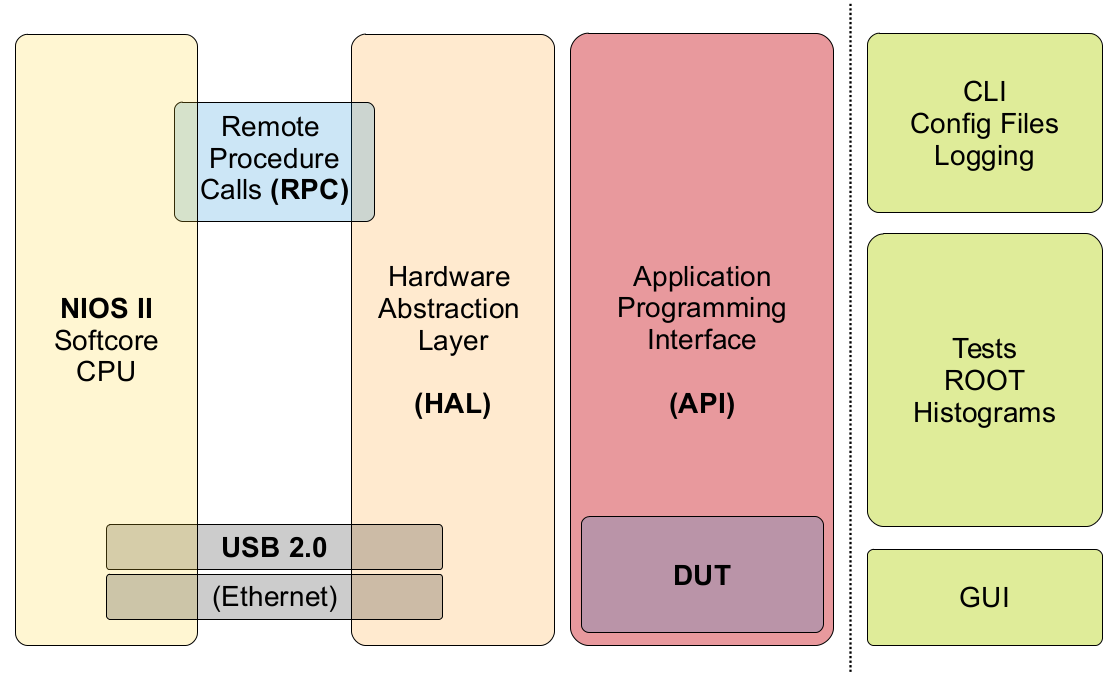
\includegraphics[width=0.95\textwidth]{pxar_scheme}
	\caption{software architecture of pXar \cite{spannagel}}
	\label{p13}
\end{figure}
% ========================================================
\subsection{\ac{HAL}}
The \ac{HAL} of the pXar-core is responsible for the direct communication with the \ac{DTB}. This is the part that has access to the RPC and USB. It supervises the data readout using pipes, which is a buffered readout of the data from the test board.\\
\hspace*{\dimexpr0.5\linewidth-5cm}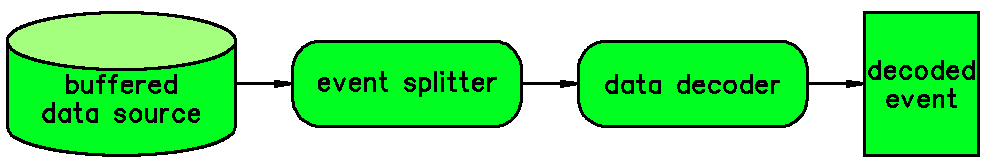
\includegraphics[width=10cm]{hal_buf}\\
The pipes can be set up for different purposes, either to deliver fully decoded events or ``raw'' events that are only split by the emulated \ac{TBM} header and trailer or complete raw data from the \ac{DTB}. The second option is very useful to debug the system, because it makes it easier to decide why something is not working. The last option may be useful for debugging too, but is mainly used for saving the raw data to a binary file.\\
Most of the basic functions with a short explanation are listed in \ar{t5}. They are loosely divided in categories i.e. basically all them can be used while the \ac{DTB} and pXar are running. So, having them in the group ``Device Initialisation'', means that they are used while initialising the board even though the may be reused afterwards.  \\
\begin{table}[ht]
	\begin{tabularx}{\textwidth}{l|X}
		\noalign{\hrule height 2pt}
		\multicolumn{2}{c}{\textbf{Device Initialisation}}							\\\noalign{\hrule height 2pt}
		\multicolumn{1}{c}{\textbf{command}}	& 	\multicolumn{1}{c}{\textbf{purpose}}	\\\hline
		initTestboard		& initialises the \ac{DTB} with its device specific \textit{signal delay} settings		\\
		setTestboardPower	& sets the \textit{analogue} and \textit{digital voltage} and \textit{current limits}		\\
		setTestboardDelays	& sets \textit{signal delay} settings		\\
		flashTestboard		& flashes a given \textit{firmware file} to the \ac{FPGA}		\\
		initROC				& initialises a \ac{ROC}s of a given \textit{type} with \textit{\ac{I2C} address} with a \textit{vector of \ac{DAC}s} 		\\
		SetupPatternGenerator	& sets the \ac{PG} to a given sequence		\\
		SetClockSource		& set clock source to internal or external		\\
		\noalign{\hrule height 2pt}
	\end{tabularx}
	\caption{base commands of \ac{HAL}}
	\label{t5}
\end{table}

\begin{table}[ht]
	\begin{tabularx}{\textwidth}{l|X}
		\noalign{\hrule height 2pt}
		\multicolumn{2}{c}{\textbf{\ac{DTB} Commands}}							\\\noalign{\hrule height 2pt}
		\multicolumn{1}{c}{\textbf{command}}	& 	\multicolumn{1}{c}{\textbf{purpose}}	\\\hline
		getTBia			& reads analogue current from \ac{DTB}		\\
		getTBva			& reads analogue voltage		\\
		getTBid			& reads digital current		\\
		getTBvd			& reads digital voltage		\\
		set*			& sets the limit of *$=$TBia, TBva, TBid, TBvd		\\
		SignalProbe*	& lays one of the internal \textit{signals} to the output *$=$D1, D2, A1, A2 		\\
		HVoff			& disables the \ac{HV} from the \ac{DTB} to the \ac{ROC}		\\
		HVon			& enables \ac{HV}		\\
		Pon 			& turns on power of the \ac{DTB}		\\
		Poff			& turns off power		\\
		rocSetDAC		& sets the \textit{\ac{DAC}} with \textit{\ac{I2C}} to a given \textit{value} 		\\
		\noalign{\hrule height 2pt}
	\end{tabularx}
	\caption{base commands of \ac{HAL}}
	\label{t6}
\end{table}

\begin{table}[ht]
	\begin{tabularx}{\textwidth}{l|X}
		\noalign{\hrule height 2pt}
		\multicolumn{2}{c}{\textbf{\ac{DAQ} Functions}}							\\\noalign{\hrule height 2pt}
		\multicolumn{1}{c}{\textbf{command}}	& 	\multicolumn{1}{c}{\textbf{purpose}}	\\\hline
		daqStart		& starts a new \ac{DAQ} session		\\
		daqTriggerSource& sets the trigger source (e.g. extern, pg)		\\
		daqTrigger		& sends out a given \textit{number} of \ac{PG} sequences with \textit{period} 		\\
		daqStop			& stop the current \ac{DAQ} session		\\
		daqEvent		& reads out a decoded event from the buffer if \ac{DAQ} is activated		\\
		daqRawEvent		& reads out a raw event		\\
		daqAllRawEvents	& reads out all events in the buffer		\\
		daqClear		& clears the buffer		\\
		\noalign{\hrule height 2pt}
	\end{tabularx}
	\caption{base commands of \ac{HAL}}
	\label{t7}
\end{table}

\begin{table}[ht]
	\begin{tabularx}{\textwidth}{l|X}
		\noalign{\hrule height 2pt}
		\multicolumn{2}{c}{\textbf{\ac{ROC} Functions}}						\\\noalign{\hrule height 2pt}
		\multicolumn{1}{c}{\textbf{command}}	& 	\multicolumn{1}{c}{\textbf{purpose}}	\\\hline
		SetupI2CValues		& sets the available \textit{\ac{I2C}} addresses		\\
		SetupTrimValues		& sets the trim bits from a given \textit{vector} for a \ac{ROC} with \textit{\ac{I2C}}		\\
		RocSetMask			& masks all pixels given in a \textit{vector}  for a \ac{ROC} with \textit{\ac{I2C}}		\\
		PixelSetCalibrate	& enables the calibrate signal for a pixel with \textit{col}, \textit{row} and \textit{\ac{I2C}}		\\
		RocClearCalibrate	& disables the calibrates for a \ac{ROC} with \textit{\ac{I2C}}		\\
		\noalign{\hrule height 2pt}
	\end{tabularx}
	\caption{base commands of \ac{HAL}}
	\label{t8}
\end{table}
% ========================================================
\subsection{\ac{API}}
The \ac{API} is the interface to the user, this is where all the commands are directed to. It is set-up in a way that it already does a lot of data pre-processing, i.e. it does assertions, range- and sanity checks for most the input parameters and commands. Thereby it is more user-friendly and a lot misusage can be avoided. To do that, it picks up the commands and functions from \ac{HAL}, the most important ones are listed in \ar{t9}\\
Included inside the \ac{API} is the self-contained \ac{DUT} class, which is responsible for the set-up of all the devices. It also saves the detector settings and makes them available all the time. The \ac{DUT} itself is initialised by the \ac{API} function initDUT($\hdots$), it is compatible with single \ac{ROC}s of both types, \ac{TBM}s or full modules. Mandatory information to start it for a single \ac{ROC} is a list of pairs of \ac{DAC}s and their values and trim bit values for all $4160$ pixels.
\begin{table}[ht]
	\begin{tabularx}{\textwidth}{l|X}
		\noalign{\hrule height 2pt}
		\multicolumn{2}{c}{\textbf{main \ac{API} functions}}						\\\noalign{\hrule height 2pt}
		\multicolumn{1}{c}{\textbf{command}}	& 	\multicolumn{1}{c}{\textbf{purpose}}	\\\hline
		initTestboard		& checks weather power setting, \ac{DTB} delays and \ac{PG} settings are viable and then start \ac{HAL} command			\\
		setDAC				& verifies that the \ac{DAC} setting are sane and then starts rocSetDAC		\\
		setExternalClock	& checks weather there is an external clock present and uses SetClockSource accordingly		\\
		daqStart			& uses daqClear, resets the mask, calibrate enable and trim settings, starts \ac{DAQ} with daqStart	from \ac{HAL}			\\
		daqStatus			& returns the status of the \ac{DAQ} 			\\
		getNEnabledPixels	& returns the number of pixels enabled for calibrates			\\
		getNMaskedPixels	& returns the number of masked pixels			\\
		getRocType			& return the \ac{ROC}-type 			\\
		testPixel			& enables the pixel with \textit{column}, \textit{row} and \textit{\ac{I2C}} and check if the pixel exists for the given \ac{ROC}			\\
		maskPixel			& masks the pixel with \textit{column}, \textit{row} and \textit{\ac{I2C}} and check if the pixel exists for the given \ac{ROC}	 			\\
		\noalign{\hrule height 2pt}
	\end{tabularx}
	\caption{base commands of \ac{API}}
	\label{t9}
\end{table}
% ========================================================
% 2
% ========================================================
\section{Decoder}
In this section I am going to describe the basic steps how the raw data from the analogue chip is decoded with pXar, which is very useful while debugging possible decoding issues and to guarantee a stable readout at all. Since pXar was made for reading out the digital chip whose \ac{ADC} is included in the \ac{ROC}, the decoding of this chip is working well and did not require any further investigation.\\
After passing the \ac{ADC} of the \ac{DTB} and the soft \ac{TBM} the raw data looks like this:
\begin{center}
\terminal{[36600, 4027, 29, 3980, 4083, 39, 90, 141, 16427]}                                                    
\end{center}
Each raw data blob consists of $16\,$bit data words of which only the last $12\,$bits contain the data, which also correspond to the output range of \ac{DTB}'s \ac{ADC}. The first four bits are used to mark the beginning and the end of a data blob. So the first step is to reduce the first four bits with a bitwise AND which sets the first four bits to zero:
\begin{equation}
	\z{dataword} = \z{dataword}\ \&\ 0\z{x}0\z{fff}\footnote{the prefix ``0x'' heralds a hexdecimal number} \equiv \z{dataword}\ \&\ \left( 2^{12} - 1\right)
\end{equation}
\begin{center}
\terminal{[3832, 4027, 29, 3980, 4083, 39, 90, 141, 43]}                                                    
\end{center}
Because the \ac{ADC} only gives out positive integers, the positive $12\,$bit range is split into two parts where the first $2^{11}$ values correspond to positive values and the second half to the negative ones. So to convert them to their negative equivalent one has to subtract the integers larger than $2^{11}$ by $2^{12}$:
\begin{equation}
	\begin{split}
		&\z{if } \z{dataword}>0\z{x}0800:\\
		&\ \ \ \ \z{dataword} = \z{dataword}\ - 0\z{x}1000 \equiv \z{dataword} - 4096
	\end{split}
\end{equation}
\begin{center}
\terminal{[-264, -69, 29, -116, -13, 39, 90, 141, 43]}                                                    
\end{center}
Now we got the values that correspond to the analogue signal. Due to various effects (e.g. different supply voltages and \ac{DAC} settings) the absolute values of the levels may vary in the whole range of the \ac{ADC}, but their spacing to one another and their offset is determined by the \ac{UB} and \ac{B} level of the \ac{ROC} header. As already mentioned in \ar{s221}, the data stream always starts with the \ac{UB} followed by the \ac{B} level of first \ac{ROC}. Even if there are more \ac{ROC} headers to come, the decoding will always take the first header in line as a reference. The distance of two address levels and their maximal deviation are defined by:
\begin{align}
	\z{level}1 &= \frac{\left( \z{\ac{B}} - \z{\ac{UB}} \right)}{4}\\
	\z{levelS} &= \frac{\left( \z{\ac{B}} - \z{\ac{UB}} \right)}{8}
\end{align}
With division is also meant a division while disregarding all non integer remainders. Level$0$ is always defined by the value of the \ac{B} level. For the example that generates the following values:
\begin{align*}
	\z{level}1 &= \frac{-69+264}{4} = 48\\
	\z{levelS} &= \frac{-69+264}{8} = 24\\
	\z{level}0 &= 0
\end{align*}
For more than one hit pXar is always averaging \ac{UB} and \ac{B} to avoid decoding errors due to random deviations.\\
To calculate the address levels the values are first corrected for an offset by subtracting level$0$, which corresponds to the $0$. After that the maximum deviation is added and the sum of both is divided by the spacing of two levels (level1).
\begin{equation}
	\z{level} = \frac{\z{dataword} - \z{level}0 + \z{levelS}}{\z{level}1} + 1
\end{equation}
The $1$ is added to make all levels positive. Through this operation only values that lie in the region -levelS/+levelS$-1$ around the middle of a spacing will be decoded correctly (q.v. \ar{p15}). The address levels of the example are $[-1, 1, 2, 3, 4]$:
\begin{center}
\terminal{[-264, -69, 29, -1, 1, 2, 3, 4, 43]}                                                    
\end{center}
Once the address levels are extracted the conversion to the pixel address follows the simple equations using the name scheme from \ar{p7}:
\begin{align}
	\z{column} &= 	2\cdot\left(  6\z{C}0 + \z{C}1 \right) + \z{CR}\mod_{2}\\
	\z{row} &= 80 - \left( 3\cdot\left(  6\z{R}0 + \z{R}1 \right) + \frac{\z{CR}}{2}\right)
\end{align}
So the example corresponds to the hit of a single pixel with the address $5/12$ (column $5$ row $12$).
\begin{figure}[ht]
	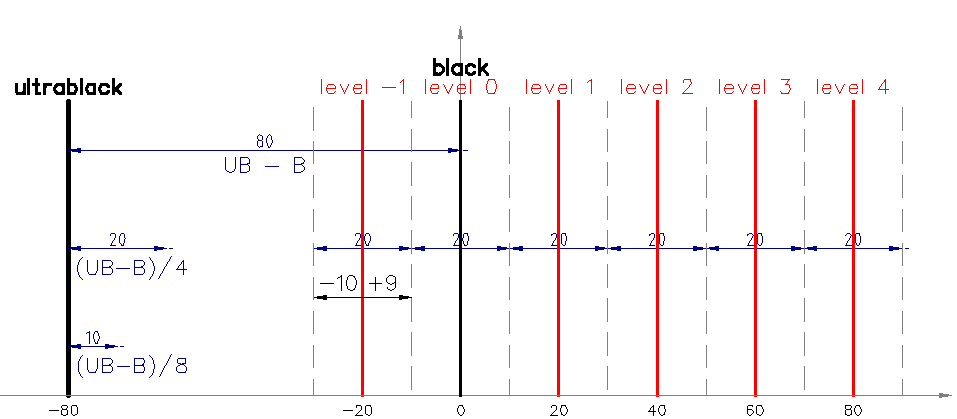
\includegraphics[width=0.95\textwidth]{decode}
	\caption{Schematic of the decoding. The red lines correspond to the ideal position of the level derived from the \ac{UB} and \ac{B}. If a measured value lies in between two dashed grey lines it will be decoded as that level.}
	\label{p15}
\end{figure}

% ========================================================
% 3
% ========================================================
\section{Pattern Generator}
The \ac{PG} is able to send out each of the four commands to the \ac{ROC}: a trigger, a  
\begin{wrapfigure}{r}{3.5cm}
	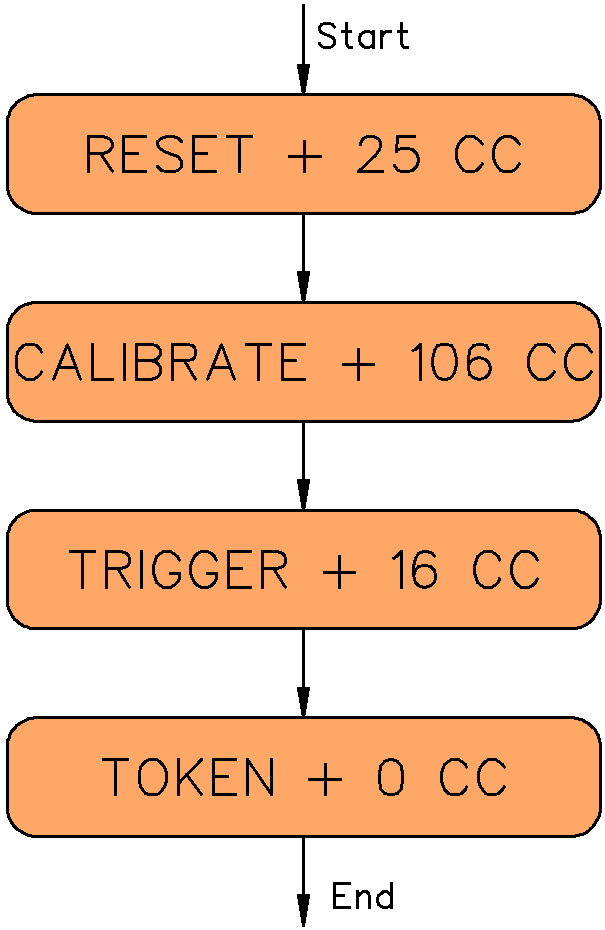
\includegraphics[width=3.4cm]{PG}
	\caption{example sequence of the \ac{PG}, CC stands for clock cycle}
	\label{p14}
\end{wrapfigure} 
token, a calibrate or a reset. A calibrate will sent out a calibration pulse to the \ac{ROC} and the reset basically deletes all hit information on the \ac{ROC}. It has a register bank with $256$ addresses at its disposal and each of these addresses can hold a single of the four commands and a delay. In that fashion there may be created arbitrary sequences of the four commands. Once the delay is set to $0$ the \ac{PG} will recognise this as a stop sign an ignore the rest of the sequence. An example is shown in \ar{p14}. This would be a basic set-up to test the functionality of the pixels. After a reset to delete all former hit information a calibrate is sent out. To read out the this event, the delay between trigger and calibrate has to be set to \textit{wbc}$+6$ to compensate for the duration the trigger needs to get to the \ac{ROC}. As the final step, the token is send out to collect the data.
% ========================================================
% 4
% ========================================================
\section{Python Interface}
Using cython most of the pXar-core functions are also accessible via python. All the available functions are listed in the cython header file \linebreak[4] ``PyPxarCore.pxd''. Should a function be amiss, it can be added to the header and the source file ``PyPxarCore.pyx`` just like in C++. So that the changes can come into effect and to use the PyPxarCore file the whole program has to be recompiled with the option ``python''.\\
Once that is done the already existing python \ac{CLI} interface ''cmdline.sh`` can be started, which initialises the \ac{DUT} in the same fashion as pXar would do it and allows to program and readout the \ac{DUT} with \ac{API}'s functions.
% ========================================================
% 4
% ========================================================
\section{Running the Software}
Once the software is properly installed meeting all the prerequisites, pXar needs a few configuration files to get started. For each \ac{ROC} that is connected to the \ac{DTB} pXar requires a file called ''dacParameters\_C$<$\ac{I2C}$>$.dat`` with all available \ac{DAC}s and corresponding start values for the respective \ac{ROC} and a file ''trimParameters\_$<$\ac{I2C}$>$.dat`` with a trim bit value for each pixel. If a completely untrimmed \ac{ROC} is required, all values have to be set to $15$, i.e. no trimming at all. Furthermore a file with delay settings for the \ac{DTB} called ''tbParameters.dat`` and a general configuration file ''configParameters.dat`` are required. Examples of these can be found in the appendix \ac{makelink}.\\
All the above files are mandatory to start the software and have to be in the same location (configuration directory). The binary files of pXar are in the directory bin of the installation folder. To run the software one has to go there and enter the command:
\begin{itemize}
	\item[$>$] ./pXar -d $<$configuration directory$>$
\end{itemize}
There are some further useful options to start the program that can be displayed using the ''-h`` option, but it will not start without ''-d``. To name the most important:
\begin{itemize}
	\item -f $<$flashfile$>$ \ka $\rightarrow$ flash a firmware from the flashfile to the \ac{FPGA} of the \ac{DTB}
	\item -g \ka $\rightarrow$ directly starts the \ac{GUI}
\end{itemize}
Since the software will start in a rather undocumented \ac{CLI} if started without the \ac{GUI} option, I recommend starting it always with the ``-g'' option as well.\\
For using the much more user specific \ac{CLI} I was always using the python version, which can be found in the python folder of the installation directory and starts with:
\begin{itemize}
	\item[$>$] ./cmdline.sh -d $<$configuration directory$>$
\end{itemize}
and is very powerful for performing and composing short tests and directly using the \ac{API} commands.
% ========================================================
% 5
% ========================================================
\section{EUDAQ}
EUDAQ is a \ac{DAQ} framework that was designed to be portable, modular and cross platform and was written in C++. It was mainly developed for the EUDET Pixel Telescope, but is very useful for other systems as well \cite{eudaq}. The program is split into different sub processes that can all run on different machines using \ac{TCP} sockets, which are shown in \ar{p16}.\\
The Run Control behaves like a central supervisor of the \ac{DAQ} and shows all the other connected processes, which is why it is the only process that has to run. All the hardware that is connected, e.g. the telescope, a \ac{TU} or other \ac{DUT}s, will have a Producer process and are thereby able to be configured, read out and to send the data to the Data Collector. The Data Collector collects the data from all Producers, combines it to a single data stream and saves it to native binary format. To keep track of potential errors there is also a Logger available that receives log messages from all processes, may receive messages from the user via the Run Control as well and saves the data in single location.\\
Thus, the reason for us using EUDAQ is quite obvious. It makes it very easy to use events off different producers and combine them into one data stream. Though there is still the urge for a trigger logic (q.v. \ar{makeref}) to keep all the events aligned. For the future the idea is to run with another Producer called \ac{TU} that can be configured in the same way as the whole trigger logic.\\
Being independent software, EUDAQ still uses the pXar-core library to operate the telescope.
\begin{figure}[ht]
	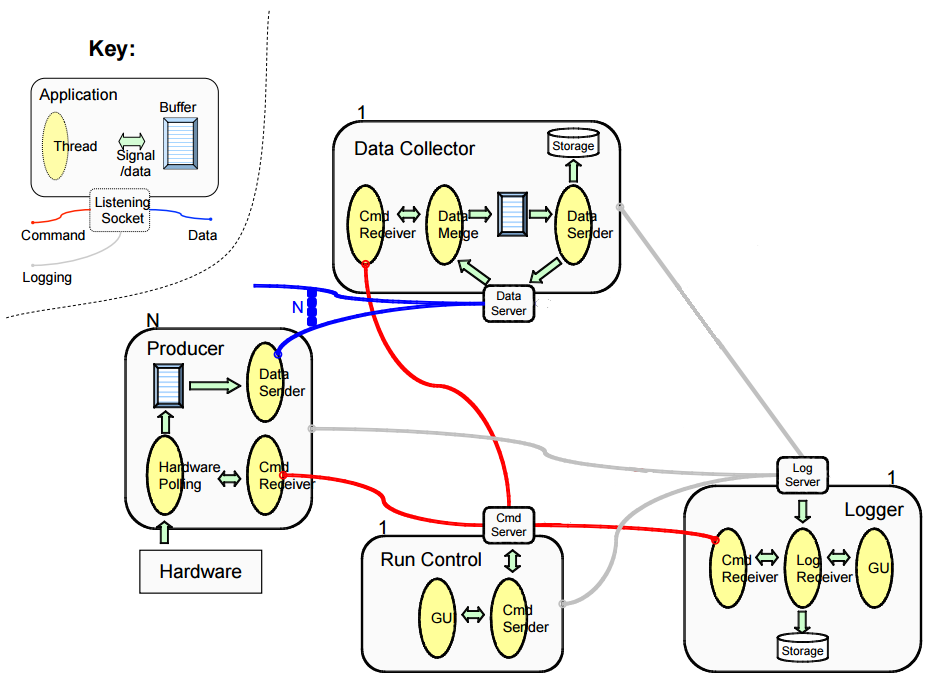
\includegraphics[width=0.95\textwidth]{eudaq}
	\caption{Schematic of the EUDAQ architecture \cite{eudaq}.}
	\label{p16}
\end{figure}

\chapter{bla}
\input{acronyms.dat}
\bibliographystyle{plain}
\bibliography{refs}
\end{document}